\lecture{18}{6. November 2025}{Deflection of Beams}

\subsection{Unsymmetric Bending}
When developing the Flexure formula above it was required that the cross-sectional area was symmetric about an axis perpendicular to the neutral axis and the resultant moment $\Vec{M}$ to act around the neutral axis. 
Now a general formula will be derived

\subsubsection{Moment applied about Principal Axis}
We consider the beam's cross section to have the unsymmetrical shape shown on \Cref{fig:f18_1}.a.
The coordinate system is placed such that the origin is located at the centroid $C$ of the cross section and the resultant moment $\Vec{M}$ acts around the $+z$ axis. 
The shear stress distribution over the entire cross sectional area must have a zero force resultant:
\[ 
0 = - \int_{\mathrm{A}} \sigma \, \mathrm{d}A
,\]
the moment of the stress distribution about $y$ must be 0:
\[ 
0 = - \int_{\mathrm{A}} z \sigma \, \mathrm{d}A
,\]
and the moment about the $z$-axis must equal $\Vec{M}$:
\[ 
M = \int_{\mathrm{A}} y \sigma \, \mathrm{d}A
.\]

\begin{figure} [ht]
  \centering
  
\includegraphics[width=0.85\linewidth]{./figures/f18_1.png}
  \caption{Moment applied about the principal axis of a beam}
  \label{fig:f18_1}
\end{figure}

The first of these equations is satisfied since the $z$-axis passes through the centroid of the area.
Also, as the $z$-axis represents the neutral axis for the cross section.
Therefore:
\[ 
0 = \frac{- \sigma_{\mathrm{max}}}{c} \int_{\mathrm{A}} yz \, \mathrm{d}A
\]
which requires
\[ 
\int_{\mathrm{A}} yz \, \mathrm{d}A = 0
.\]

The above integral is called the \textit{product of inertia} for the area. 
This will always be zero so long as the $y$ and $z$ axes are chosen as the principal axes of inertia for the area.


\subsubsection{Moment Arbitrarily Applied}
Sometimes a member will be loaded such that $\Vec{M}$ does not act about one of the principal axes of the cross section. 
When this occurs, the moment should first be resolved into components along the principal axes, then the flexure formula can be used to determine the normal stress caused by each component. 
Finally, the principle of superposition can be applied to find the resultant normal stress at the point.

That is:
\begin{equation} \label{eq:1117}
  \sigma = - \frac{M_z y}{I_z} + \frac{M_y z}{I_y}
\end{equation}


\subsubsection{Orientation of the Neutral Axis}
\begin{figure} [ht]
  \centering
  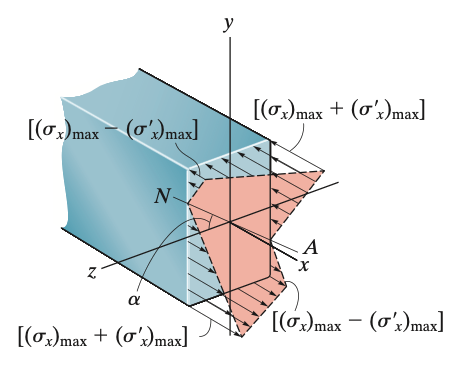
\includegraphics[width=0.4\linewidth]{./figures/f18_2.png}
  \caption{The orientation of the neutral axis.}
  \label{fig:f18_2}
\end{figure}

The equation defining the neutral axis and its inclination $\alpha$, from \Cref{fig:f18_2}, can be determined by applying \Cref{eq:1117} to a point $0, y, z$ where $\sigma = 0$, which gives:
\[ 
y = \frac{M_y I_z}{M_z I_y} z
.\]
Since $M_z = M \cos \theta$ and $M_y = M \sin \theta$ then
\[ 
y = \left( \frac{I_z}{I_y} \tan \theta \right) z
.\]
The slope of the neutral axis is $\tan \alpha = y / z$, hence:
\[ 
\tan \alpha = \frac{I_z}{I_y} \tan \theta
.\]


\section{Deflection of Beams and Shafts}

\subsection{The Elastic Curve}
We consider the beam shown on \Cref{fig:f18_3}.a and remove the small element located at distance $x$ from the left end and having an undeformed length of $\mathrm{d} x$. 
On \Cref{fig:f18_3}.b the localized $y$-coordinate is measured from the elastic curve (neutral axis) to the fiber in the beam that has an original length of $\mathrm{d}s = \mathrm{d}x$  and a deformed length $\mathrm{d}s'$.

\begin{figure} [ht]
  \centering
  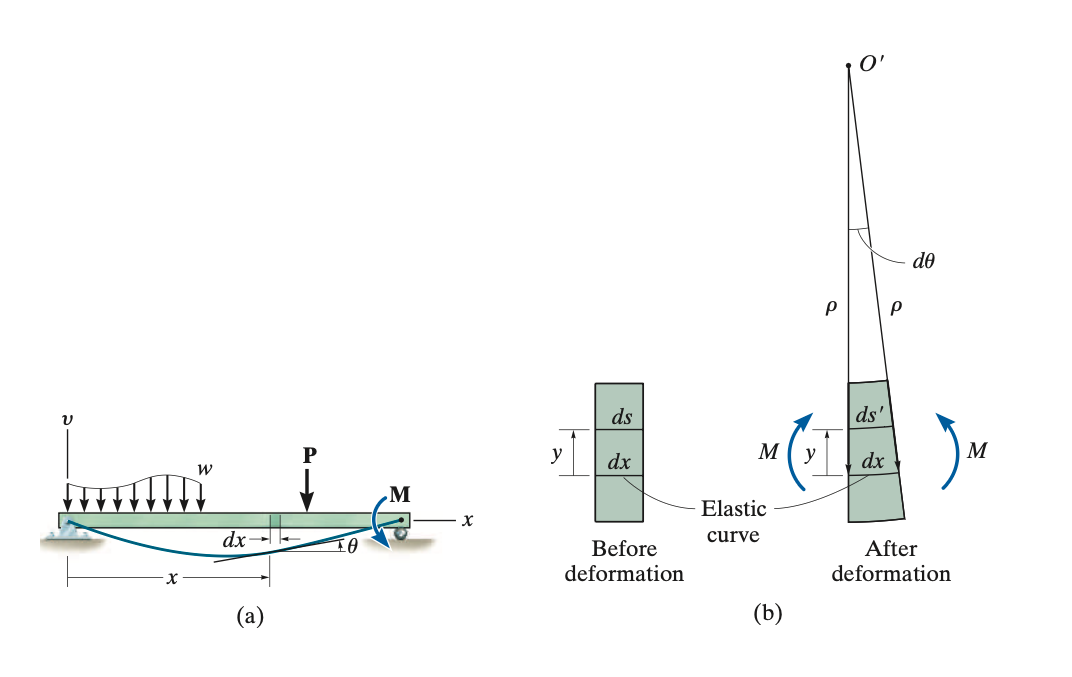
\includegraphics[width=0.85\linewidth]{./figures/f18_3.png}
  \caption{Moment-curvature relationsip in a beam.}
  \label{fig:f18_3}
\end{figure}

From Hooke's law we can obtain
\[ 
\frac{1}{\rho} = \frac{M}{EI}
.\]
Where:
\begin{center}
  \begin{tabular}{ll}
    $\rho$ & The radius of curvature at the point \\
    $M$ & The internal moment in the beam at the point \\
    $E$ & The modulus of elasticity of the material \\
    $I$ & The moment of inertia about the neutral axis of the beam
  \end{tabular}
\end{center}

\subsection{Slope and Displacement by Integration}
For most problems the \textit{flexural rigidity} ($EI$) is constant along the length of the beam.
Assuming this is the case we obtain:
\begin{align*}
  EI \frac{\mathrm{d}^{4}v}{\mathrm{d}x^{4}}  &= w(x) \\
  EI \frac{\mathrm{d}^3v}{\mathrm{d}x^3} &= V(x) \\
  EI \frac{\mathrm{d}^2 v}{\mathrm{d}x^2}  &= M(x)
.\end{align*}


\subsubsection{Boundary Conditions}
Solving any of these equations requires successive integrations to obtain $v$.
For each integration, a constant of integration is introduced and one must therefore solve for all these constants to obtain a unique solution for a particular problem.

